\documentclass[aspectratio=169]{beamer} % O parâmetro aspectratio com valar 16:9 deixa o slide em widescreen

\usepackage[brazil]{babel}
\usepackage[utf8]{inputenc}
\usepackage[T1]{fontenc}

\usetheme{Madrid}
\setbeamertemplate{navigation symbols}{}

\title[Educação em Tecnologias Digitais]{Educação em Tecnologias Digitais}

\author[Diego S. C. Nascimento]{Diego Silveira Costa Nascimento}

\institute[IFRN]{
Instituto Federal de Educação, Ciência e Tecnologia do Rio Grande do Norte\\
diego.nascimento@ifrn.edu.br
}

\date[\today]{\today}

\begin{document}

\begin{frame}[plain]
	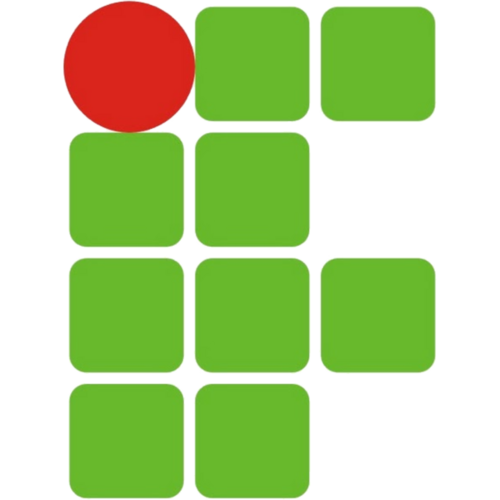
\includegraphics[scale=0.2]{img/IFRN}
	\titlepage
\end{frame}

\logo{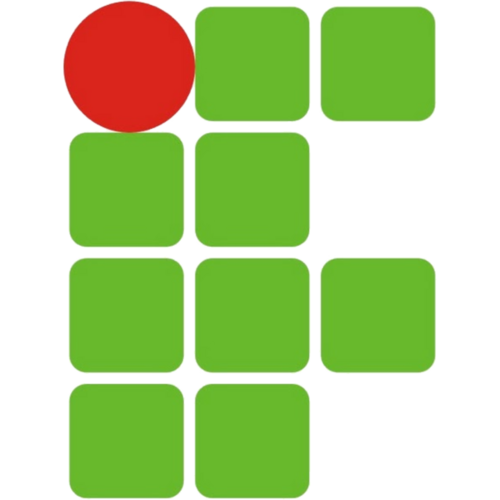
\includegraphics[scale=0.1]{img/IFRN}}

\begin{frame}
	\frametitle{Ementa}
  	\tableofcontents
\end{frame}

\AtBeginSection[]{
	\begin{frame}
		\frametitle{Ementa}
		\tableofcontents[currentsection]
	\end{frame}
}

\section{Sistemas Operacionais}

\begin{frame}
	\frametitle{Sistema Operacional}
	
	\begin{itemize} 
		\item É o software fundamental que gerencia o hardware e os recursos do computador;
		\item Fornece serviços essenciais para outros programas; e
		\item Atua como uma ponte entre o usuário e o hardware do computador, facilitando a execução de tarefas e a operação de aplicativos.
	\end{itemize}\vfill
	
	\begin{exampleblock}{Exemplos}
		\begin{itemize}
			\item Windows;
			\item Linux;
			\item MacOS; e
			\item Chrome OS.
		\end{itemize}
	\end{exampleblock}
\end{frame}

\begin{frame}
	\frametitle{Principais Funções}
	
	\begin{itemize}
		\item Gerenciamento de processos;
		\item Gerenciamento de memória;
		\item Gerenciamento de recursos;
		\item Entrada e saída de dados; e
		\item Sistema de arquivos.
	\end{itemize}
\end{frame}

\begin{frame}
	\frametitle{Windows}
	
	\begin{itemize}
		\item Teve a primeira versão lançada em 1985; e
		\item É uma família de sistemas operacionais comercializados e vendidos pela Microsoft.
	\end{itemize}\vfill
	
	\begin{center}
		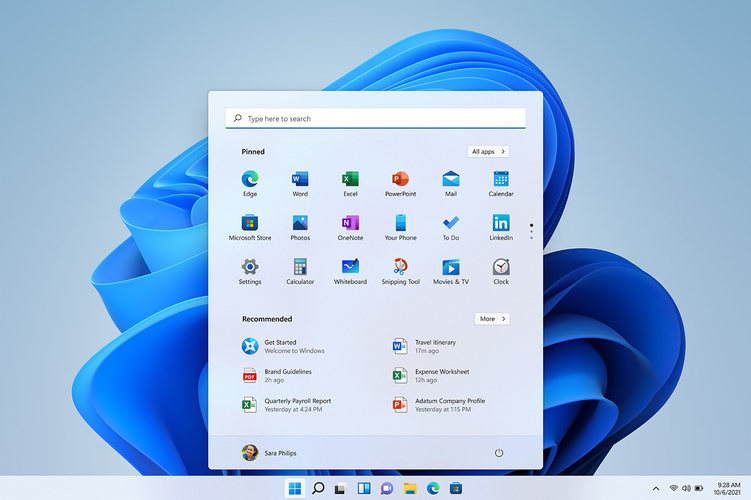
\includegraphics[scale=1]{img/windows11}
	\end{center}
\end{frame}

\begin{frame}
	\frametitle{Linux}
	
	\begin{itemize}
		\item Foi desenvolvido pelo programador finlandês Linus Torvalds, inspirado no sistema Minix; 
		\item Teve a primeira versão lançada em 1991; e
		\item O código-fonte está disponível sob a licença GPL (versão 2) para que qualquer pessoa o possa utilizar, estudar, modificar e distribuir livremente.
	\end{itemize}\vfill
	
	\begin{center}
		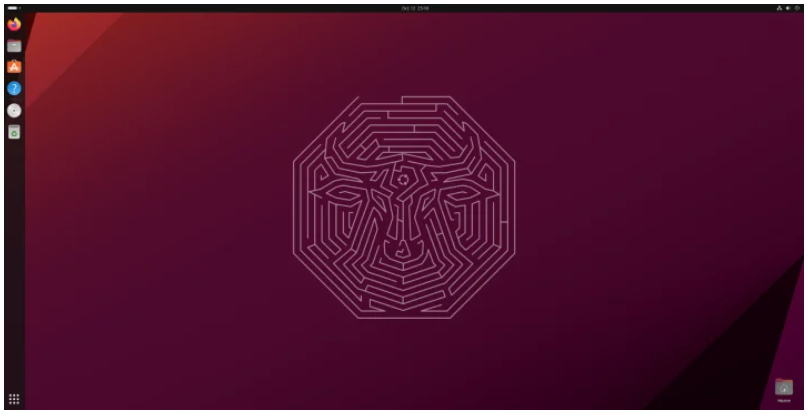
\includegraphics[scale=0.4]{img/ubuntu2310}
	\end{center}
\end{frame}

\begin{frame}
	\frametitle{Mac OS}
	
	\begin{itemize}
		\item É um sistema operacional proprietário desenvolvido e distribuído pela Apple;
		\item Teve a primeira versão lançada em 1984.
	\end{itemize}\vfill
	
	\begin{center}
		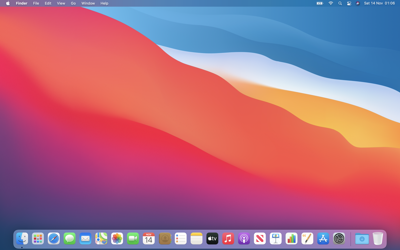
\includegraphics[scale=0.45]{img/macosbig}
	\end{center}
\end{frame}

\begin{frame}
	\frametitle{Chrome OS}
	
	\begin{itemize}
		\item É um sistema operacional desenvolvido pelo Google;
		\item Teve a primeira versão lançada em 2010; e
		\item É baseado no núcleo do Linux. 
	\end{itemize}\vfill
	
	\begin{center}
		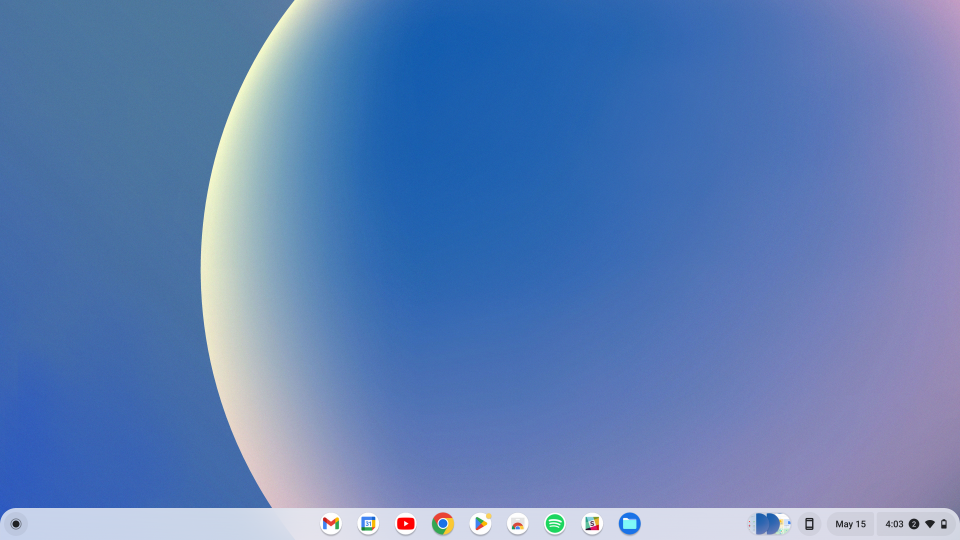
\includegraphics[scale=0.2]{img/chromeos}
	\end{center}
\end{frame}

\begin{frame}
	\frametitle{Área de Trabalho}
	
	\begin{itemize}
		\item É a tela principal que é exibida ao ligar o computador;
		\item Possibilita o acesso a ícones, arquivos, pastas e programas;
		\item É como uma superfície de uma mesa onde você organiza seus itens de trabalho; e
		\item Pode ser personalizada com papéis de parede, atalhos e widgets para facilitar o acesso às suas ferramentas e documentos mais usados.
	\end{itemize}
\end{frame}

\begin{frame}
	\frametitle{Barra de Tarefas}
	
	\begin{itemize}
		\item Geralmente localizada na parte inferior da tela;
		\item Permite que você acesse e gerencie rapidamente programas e funções do sistema; e
		\item Componentes:
		\begin{itemize}
			\item Botão iniciar;
			\item Barra de pesquisa;
			\item Ícones de aplicativos;
			\item Área de notificação; e
			\item Relógio e data.
		\end{itemize}
	\end{itemize}
\end{frame}

\begin{frame}
	\frametitle{Menu}
	
	\begin{itemize}
		\item Também conhecido como menu Iniciar no Windows;
		\item É uma ferramenta que permite acessar rapidamente os programas instalados no seu computador;
		\item Geralmente está localizado no canto inferior esquerdo da tela; e
		\item Pode ser aberto pressionando a tecla Windows no teclado.
	\end{itemize}
\end{frame}

\begin{frame}
	\frametitle{Lixeira}
	
	\begin{itemize}
		\item É um recurso que armazena temporariamente os arquivos e pastas que foram excluídos; e
		\item Permite a recuperação de arquivos deletados acidentalmente.
	\end{itemize}
\end{frame}

\begin{frame}
	\frametitle{Janela}
	
	\begin{itemize}
		\item Barra de título;
		\item Menu;
		\item Minimizar;
		\item Maximizar/Restaurar; e
		\item Fechar.
	\end{itemize}
\end{frame}

\begin{frame}
	\frametitle{Gerenciador de Arquivos}
	
	\begin{itemize}
		\item É um programa que permite visualizar, organizar e manipular os arquivos e pastas no seu computador;
		\item Facilita tarefas como copiar, mover, renomear e excluir arquivos; e
		\item Permite a criação de novas pastas e a busca por documentos específicos.
	\end{itemize}
\end{frame}

\begin{frame}
	\frametitle{Configurações do Sistema}
	
	\begin{itemize}
		\item São um conjunto de opções que permitem personalizar e ajustar o funcionamento do seu computador;
		\item Permite modificar aspectos do sistema operacional, como a aparência, rede, segurança e o hardware; e
		\item Pode ser acessado clicando no ícone de engrenagem no menu Iniciar.
		\item Áreas comuns:
		\begin{itemize}
			\item Sistema: Ajustes de tela, notificações, energia e armazenamento;
			\item Dispositivos: Configurações de impressoras, mouses, teclados e outros dispositivos conectados;
			\item Rede e Internet: Configurações de Wi-Fi, Ethernet e VPN;
			\item Personalização: Alterar o papel de parede, temas e a barra de tarefas;
			\item Contas: Gerenciar contas de usuário e opções de login; e
			\item Atualização e Segurança: Verificar atualizações do sistema e ajustar configurações de segurança.
		\end{itemize}
	\end{itemize}
\end{frame}

\begin{frame}
	\frametitle{Encerramento do Sistema}
	
	\begin{itemize}
		\item Suspender;
		\item Reiniciar; e
		\item Desligar.
	\end{itemize}
\end{frame}

\begin{frame}
	\frametitle{Softwares Utilitários}
	
	\begin{itemize}
		\item São programas que ajudam a gerenciar, manter e otimizar o funcionamento do seu computador; e
		\item Eles realizam tarefas específicas que garantem que o sistema operacional e os dispositivos funcionem de maneira eficiente.
	\end{itemize}\vfill
	
	\begin{exampleblock}{Exemplos}
		\begin{itemize}
			\item Compactadores de arquivos;
			\item Antivírus;
			\item Ferramenta de backups; e
			\item Desfragmentador de disco.
		\end{itemize}
	\end{exampleblock}
\end{frame}

\begin{frame}
	\frametitle{Compacta\c cão de Arquivos}
	
	\begin{itemize}
		\item São programas que reduzem o tamanho de arquivos e pastas, facilitando o armazenamento e a transferência; e
		\item Eles utilizam algoritmos de compressão para diminuir o espaço ocupado pelos dados, sem perder informações.
	\end{itemize} \vfill
	
	\begin{exampleblock}{Exemplos}
		\begin{itemize}
			\item 7-Zip;
			\item WinZip; e
			\item WinRAR.
		\end{itemize}
	\end{exampleblock}
\end{frame}

\begin{frame}
	\frametitle{Antivírus}
	
	\begin{itemize}
		\item É um software projetado para detectar, prevenir e remover malware, como vírus, worms, trojans, spyware e outros tipos de ameaças cibernéticas; e
		\item Ele monitora constantemente o sistema em busca de atividades suspeitas e realiza verificações periódicas para garantir que seu computador esteja protegido.
	\end{itemize}\vfill

	\begin{exampleblock}{Programas}
		\begin{itemize}
			\item McAfee;
			\item Microsoft Defender;
			\item Avast;
			\item AVG.
		\end{itemize}
	\end{exampleblock}
\end{frame}

\begin{frame}
	\frametitle{Backup de Arquivos}
	
	\begin{itemize}
		\item É o processo de criar cópias de segurança dos seus dados para protegê-los contra perda ou danos;
		\item Essas cópias podem ser armazenadas em diferentes locais, como discos rígidos externos, servidores na nuvem ou outros dispositivos de armazenamento;
		\item O objetivo é garantir que você possa recuperar seus dados em caso de falhas no sistema, ataques de malware, exclusão acidental ou outros problemas.
	\end{itemize}
\end{frame}

\begin{frame}
	\frametitle{Desfragmentador de Arquivos}
	
	\begin{itemize}
		\item É uma ferramenta de software que reorganiza os dados no disco rígido para que os arquivos sejam armazenados de maneira contígua;
		\item Isso melhora a eficiência do acesso aos dados e, consequentemente, o desempenho do computador; e
		\item Com o tempo, à medida que você adiciona, modifica e exclui arquivos, os dados podem se espalhar pelo disco, causando fragmentação.
	\end{itemize}
\end{frame}

\section{Internet}

\begin{frame}
	\frametitle{Internet}
	
	\begin{block}{Defini\c cão}
		É uma rede global de dispositivos interconectados que permite a comunicação instantânea e o acesso a uma vasta quantidade de informações.
	\end{block}
\end{frame}

\begin{frame}
	\frametitle{Como Funciona?}
	
	\begin{itemize}
		\item A Internet funciona por meio de protocolos de comunicação;
		\item O protocolo padrão é o TCP/IP;
		\item Os dados são transmitidos por meio de roteadores e servidores em todo o mundo; e
		\item Os dados são transmitido por meio de pacotes.
	\end{itemize}
\end{frame}

\begin{frame}
	\frametitle{Benefícios}
	
	\begin{itemize}
		\item Acesso à informação em tempo real;
		\item Comunicação fácil e instantânea; e
		\item Compartilhamento de recursos e colaboração global.
	\end{itemize}
\end{frame}

\begin{frame}
	\frametitle{História}
	
	\begin{itemize}
		\item Início da década de 1960: a partir de pesquisas militares, no períodos, da Guerra Fria, começam a surgir os primeiros esboços da internet;
		\item 1969: DARPA (Department Advanced Reseach and Projects Agency) patrocinou o projeto que mais tarde seria chamado ARPANET;
		\item Início de 1983: ARPANET adota o protocolo TCP/IP;
		\item 1985: NSF (National Science Foundation) interliga seus supercomputadores formando a NSFnet.
		\item 1986: NSFnet conecta-se ao ARPANET e passa a ser chamada de Internet;
		\item 1989: Comunidade acadêmica Rio-São Paulo (Fadesp + LNCC/UFRJ) se liga a Internet;
	\end{itemize}
\end{frame}

\begin{frame}
	\frametitle{História}
	
	\begin{itemize}
		\item 1992: O cientista Tim Berners-Lee, do CERN, criou a World Wide Web – www;
		\item 1993: A Internet passa a ser explorada comercialmente no EUA e em outros países;
		\item A Internet tem seu sucesso fora do mundo acadêmico graças à distribuição do Mosaic, o primeiro navegador para a Web; e
		\item 1994: A Internet passa a ser explorada comercialmente no Brasil; e Sai a primeira versão do Netscape Navigator.
	\end{itemize}
\end{frame}

\begin{frame}
	\frametitle{O que é uma página?}
	
	\begin{block}{Defini\c cão}
		É uma coleção específica de informações (textos, imagens, vídeos, e outros arquivos multimídia) fornecidas por um site e exibidas a um usuário em um navegador web.
	\end{block} \vfill

	\begin{center}
		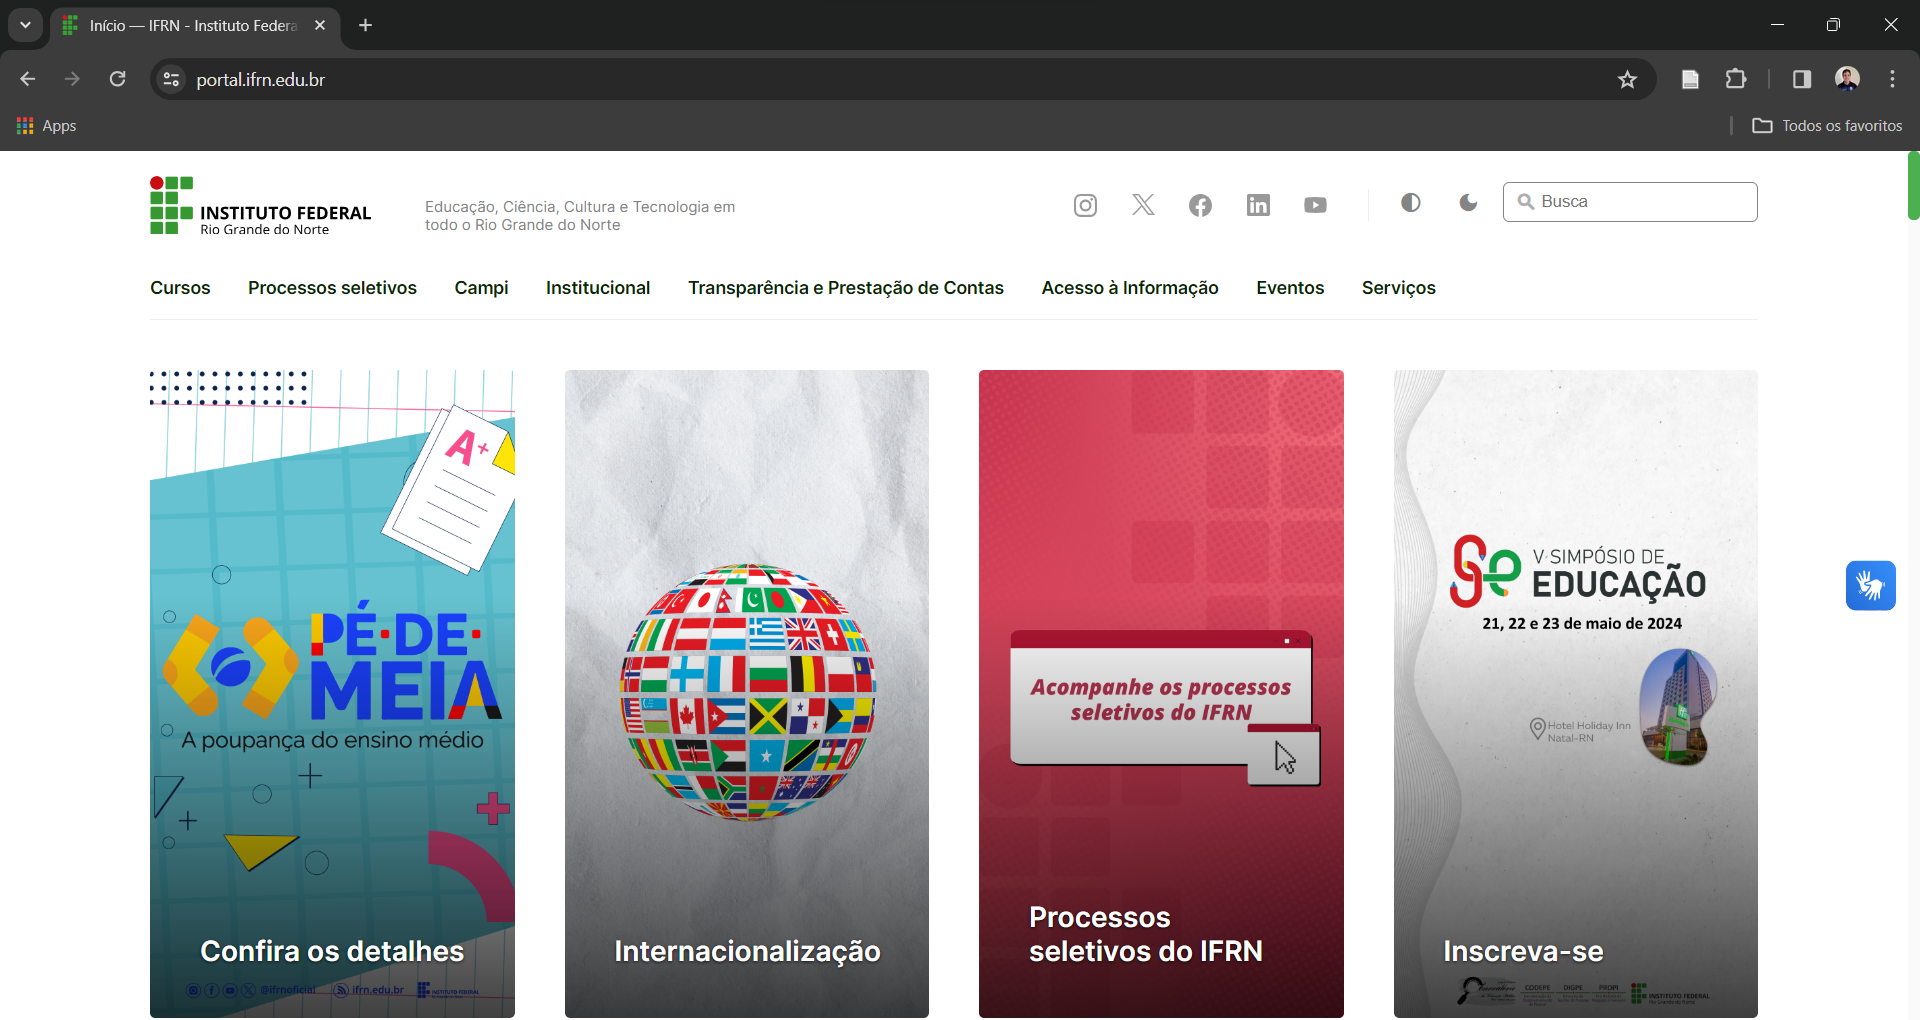
\includegraphics[scale=0.13]{img/pagina}
	\end{center}
\end{frame}

\begin{frame}
	\frametitle{O que é URL?}
	
	\begin{block}{Defini\c cão}
		É o endereço virtual de uma página ou website.
	\end{block} \vfill
	
	\begin{itemize}
		\item Um acrônimo para \underline{U}niform \underline{R}esource \underline{L}ocator;
		\item Está divida em: 
		\begin{enumerate}
			\item Protocolo; 
			\item Subdomínio;
			\item Domínio; e 
			\item Subdiretórios.
		\end{enumerate}				
	\end{itemize} \vfill
	
	\begin{exampleblock}{Exemplo}
		\begin{center}
			$\underbrace{http}_{1}$://$\underbrace{www}_{2}$.$\underbrace{ifrn.edu.br}_{3}$/$\underbrace{campus/natalcentrohistorico/}_{4}$
		\end{center}
	\end{exampleblock}
\end{frame}

\begin{frame}
	\frametitle{Navegador}
	
	\begin{block}{Defini\c cão}
		É um programa que habilita seus usuários a interagirem com documentos HTML hospedados em um servidor da rede.
	\end{block} \vfill
	
	\begin{exampleblock}{Exemplos}
		\begin{itemize}
			\item Google Chrome;
			\item Mozilla Firefox;
			\item Microsoft Egde;
			\item Safari;
			\item Opera; e
			\item Brave.
		\end{itemize}
	\end{exampleblock}
\end{frame}

\begin{frame}
	\frametitle{Entendendo o Navegador}
	
	\begin{itemize}
		\item Barra de endereço;
		\item Abas;
		\item Favoritos; e
		\item Janela anônima.
	\end{itemize}
\end{frame}

\begin{frame}
	\frametitle{Correio Eletrônico}
	
	\begin{block}{Defini\c cão}
		É uma tecnologia que permite compor, enviar e receber mensagens através de sistemas eletrônicos de comunicação assíncrona.
	\end{block}
\end{frame}

\begin{frame}
	\frametitle{O que é endere\c co de e-mail?}
	
	\begin{block}{Defini\c cão}
		É o endere\c co postal na internet.
	\end{block} \vfill
	
	\begin{itemize}
		\item Está divida em: 
		\begin{enumerate}
			\item Nome do utilizador; 
			\item Símbolo;  e
			\item Domínio. 
		\end{enumerate}				
	\end{itemize} \vfill
	
	\begin{exampleblock}{Exemplo}
		\begin{center}
			$\underbrace{exemplo}_{1}$ $\underbrace{@}_{2}$ $\underbrace{ifrn.edu.br}_{3}$
		\end{center}
	\end{exampleblock}
\end{frame}

\begin{frame}
	\frametitle{Organiza\c cão do correio eletrônico}
	
	\begin{itemize}
		\item Caixa de entrada;
		\item Enviados;
		\item Rascunhos;
		\item Excluídos; e
		\item Spam.
	\end{itemize}
\end{frame}

\begin{frame}
	\frametitle{Composi\c cão da Mensagem}
	
	\begin{itemize}
		\item Destinatário;
		\item Assunto;
		\item Corpo do e-mail; e
		\item Anexos.
	\end{itemize}
\end{frame}

\begin{frame}
	\frametitle{Armazenamento em Nuvem}
	
	\begin{block}{Defini\c cão}
		É um serviço de armazenamento e sincronização de arquivos a partir de qualquer computador ou outros dispositivos compatíveis ligados à internet.
	\end{block} \vfill
	
	\begin{exampleblock}{Exemplos}
		\begin{itemize}
			\item Google Drive;
			\item OneDrive;
			\item iCloud; 
			\item Dropbox; e
			\item Amazon Cloud.
		\end{itemize}
	\end{exampleblock}
\end{frame}

\begin{frame}
	\frametitle{Utilizando o armazenamento em nuvem}
	
	\begin{itemize}
		\item Criando/Carregando pasta;
		\item Criando/Carregando arquivo; e
		\item Realizando compartilhamento.
	\end{itemize}
\end{frame}

\section{Ambiente Virtual de Aprendizagem}

\begin{frame}
	\frametitle{AVA}
	
	\begin{itemize}
		\item É uma plataforma online que oferece suporte ao processo de ensino e aprendizagem;
		\item Permitindo que alunos e professores interajam, compartilhem conteúdos e realizem atividades; e
		\item Possibilita o acompanhamento do progresso educacional de forma digital.
	\end{itemize} \vfill
	
	\begin{exampleblock}{Exemplos}
		\begin{itemize}
			\item Google Sala de Aula;
			\item Moodle; e
			\item Blackboard.
		\end{itemize}
	\end{exampleblock}
\end{frame}

\begin{frame}
	\frametitle{Características}
	
	\begin{itemize}
		\item Acesso remoto: Pode ser acessado de qualquer lugar com conexão à internet.
		\item Materiais didáticos: Disponibilização de textos, vídeos, apresentações, links e outros recursos.
		\item Atividades e avaliações: Exercícios, fóruns, quizzes, provas e tarefas.
		\item Comunicação: Fóruns, chats, mensagens internas e videoconferências.
		\item Acompanhamento: Relatórios de desempenho, frequência e progresso dos alunos.
	\end{itemize}
\end{frame}

\begin{frame}
	\frametitle{Benefícios}
	
	\begin{itemize}
		\item Acessibilidade: possibilita o acesso ao conteúdo a qualquer momento e de qualquer lugar;
		\item Flexibilidade: permite o aprendizado em um ritmo personalizado;
		\item Interação e colaboração: facilita a comunicação entre alunos e professores, além da troca de experiências entre os próprios alunos;
		\item Diversidade de recursos: oferece diferentes formatos de conteúdo para atender às necessidades dos alunos.
	\end{itemize}
\end{frame}

\begin{frame}{Google Sala de Aula}
	
	\begin{itemize}
		\item É uma plataforma gratuita desenvolvida pelo Google;
		\item Facilita a gestão de aulas online;
		\item Integra diversas ferramentas do Google Workspace:
		\begin{itemize}
			\item Google Drive;
			\item Google Documentos;
			\item Google Meet; e 
			\item Google Calendário.
		\end{itemize}
		\item Proporciona um ambiente virtual de aprendizagem simples e eficiente; e
		\item Pode ser acessado pelo navegador, celular ou tablet.
	\end{itemize}
\end{frame}

\begin{frame}{Turmas}
	
	\begin{itemize}
		\item São os espaços virtuais criados pelos professores; e
		\item São exibidas no formato de cartões.
	\end{itemize}\vfill
	
	\begin{center}
		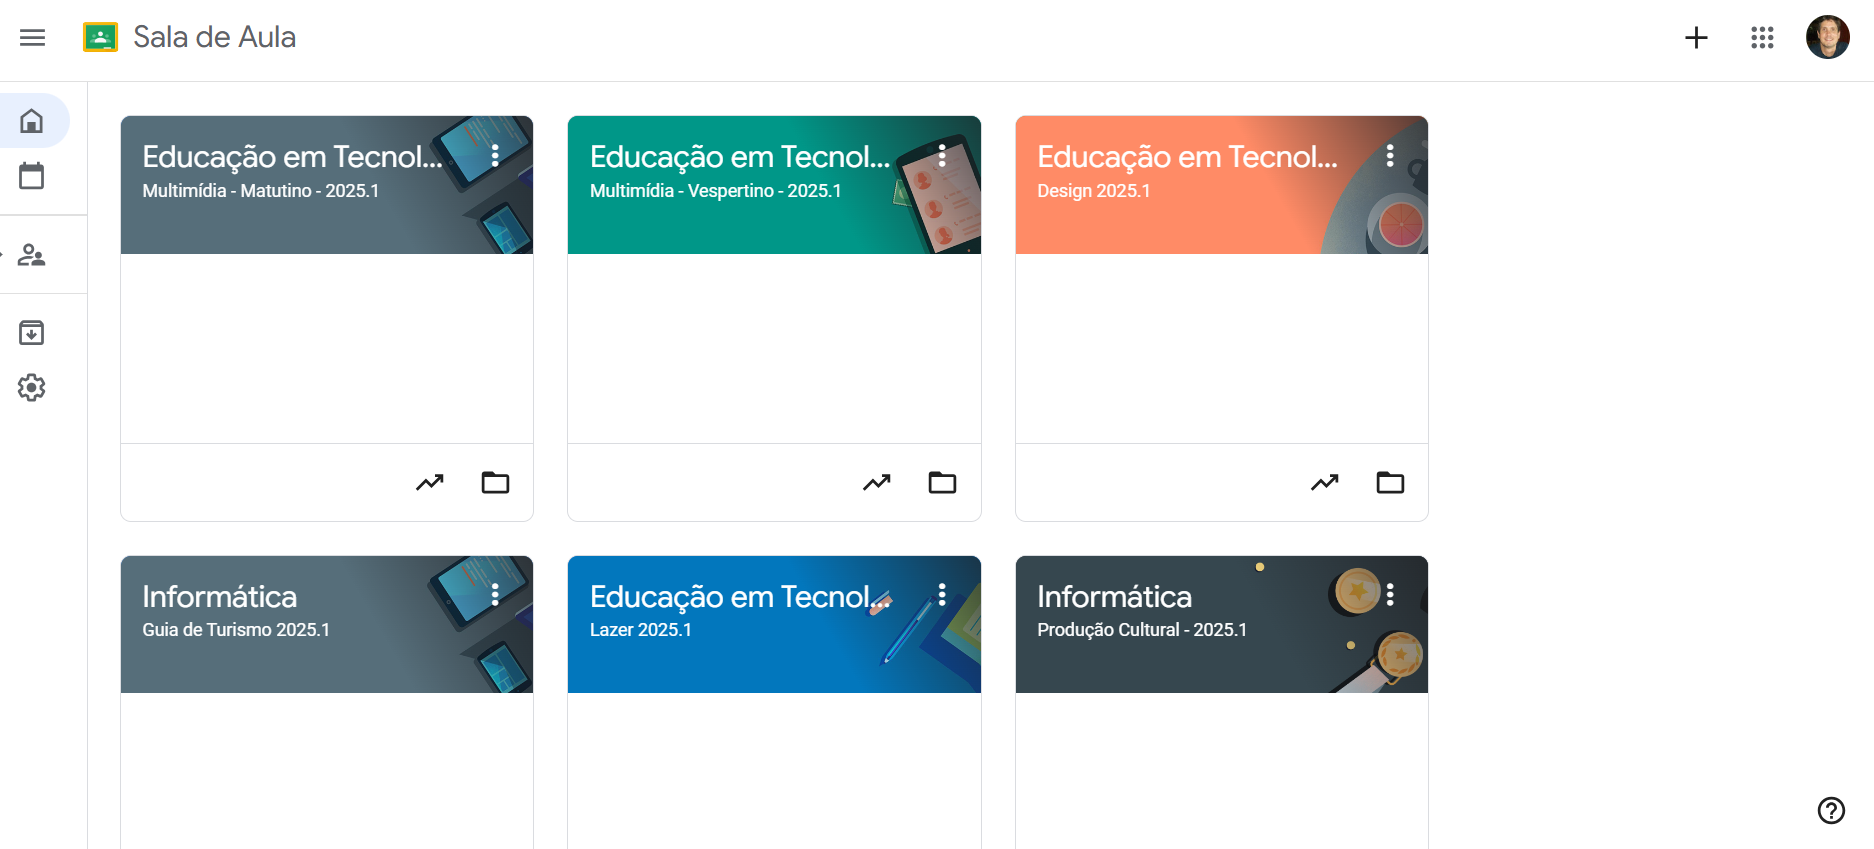
\includegraphics[scale=0.2]{img/sga}
	\end{center}
\end{frame}

\begin{frame}{Organização de uma turma}
	
	\begin{itemize}
		\item Mural: espaço para avisos e comunicações;
		\item Atividades: onde ficam tarefas, materiais e tópicos;
		\item Pessoas: lista de professores e alunos; e
		\item Notas: acompanhamento do desempenho dos alunos.
	\end{itemize}\vfill
	
	\begin{center}
		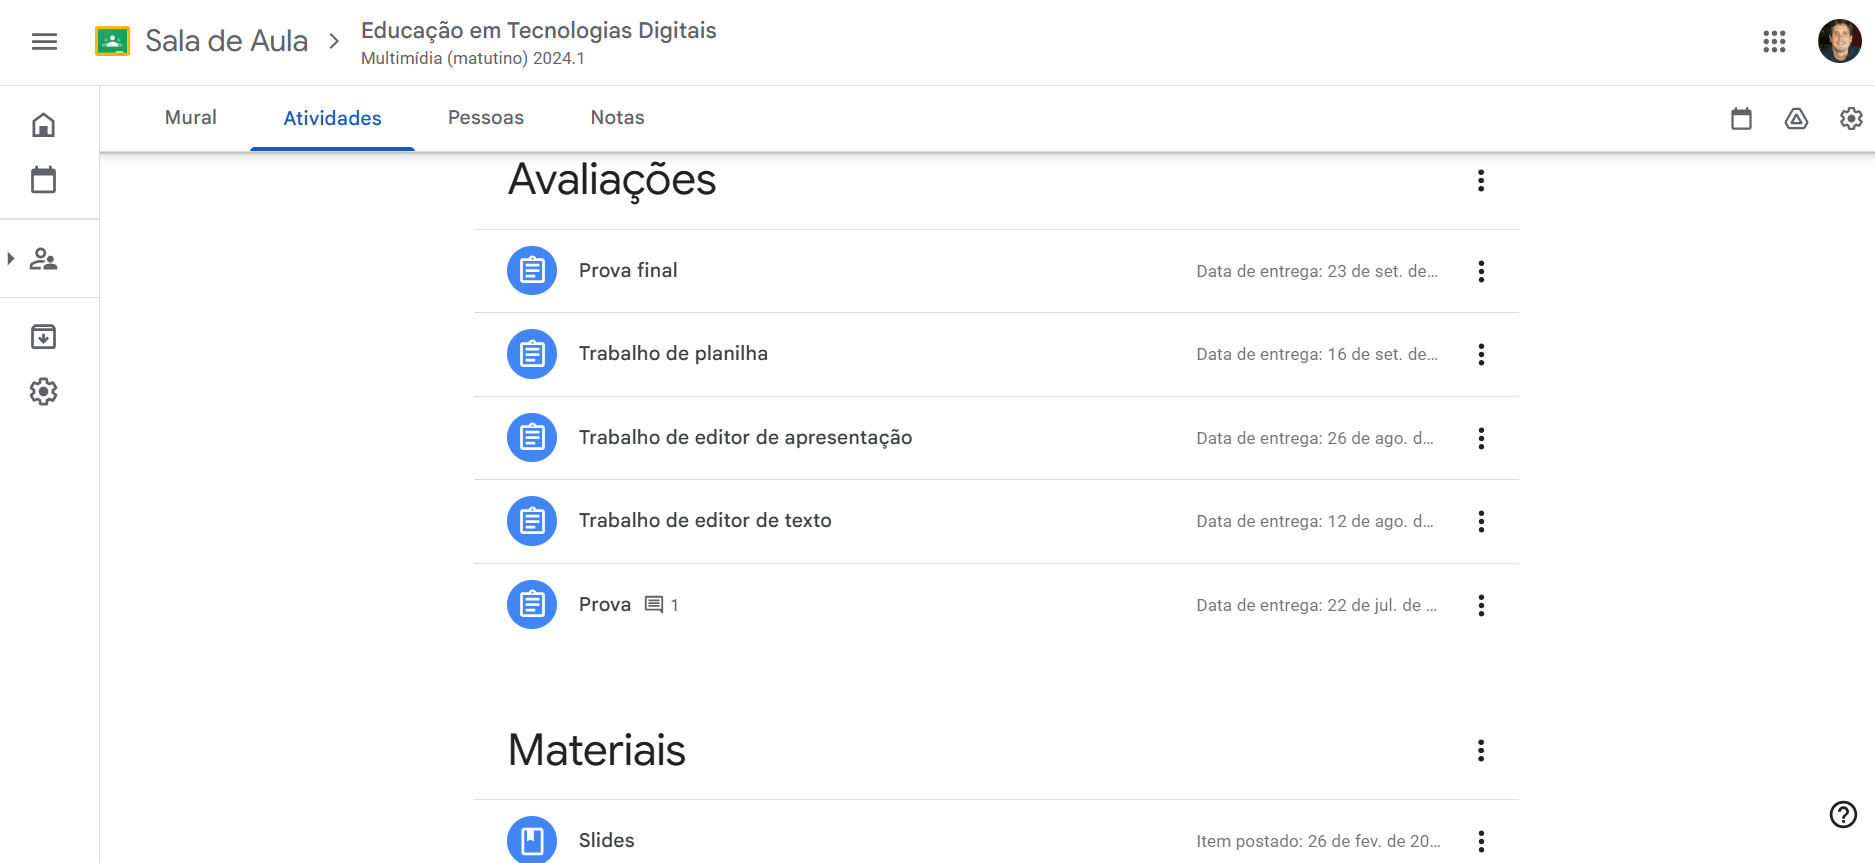
\includegraphics[scale=0.2]{img/turma}
	\end{center}
\end{frame}

\begin{frame}{Como acessar?}
	
	\begin{itemize}
		\item Link de inscrição:
		\begin{enumerate}
			\item Acesse o SUAP;
			\item Escolha no menu a opção \underline{Ensino};
			\item Escolha a opção \underline{Minhas Disciplinas};
			\item Na disciplina escolha \underline{Ambiente Virtual}.
		\end{enumerate}
		\item Código da turma:
		\begin{enumerate}
			\item Acesse o Google sala de aula;
			\item Acesse o botão $+$ no canto superior direito da tela;
			\item Escolha \underline{Participar da turma};
			\item Informe o código da turma fornecido pelo professor(a);
			\item Clique em \underline{Participar}.
		\end{enumerate}
	\end{itemize} \vfill
	
	\alert{É necessário usar sua conta @escolar.ifrn.edu.br}
\end{frame}


\section{Segurança da Informação}

\begin{frame}
	\frametitle{Segurança da Informação}
	
	\begin{block}{Definição}
		 É uma série de ações adotadas estrategicamente para controlar e evitar riscos de roubo, danos e perdas dos dados, dispositivos, servidores, sistemas e redes.
	\end{block}
\end{frame}

\begin{frame}
	\frametitle{Pilares da Segurança da Informação}

	\begin{itemize}
		\item Confiabilidade;
		\item Integridade; e
		\item Disponibilidade.
	\end{itemize}
\end{frame}

\begin{frame}
	\frametitle{Ameaças à Segurança da Informação}
	
	\begin{itemize}
		\item Malware;
		\item Phishing;
		\item Ataques de DDoS; e
		\item Engenharia Social.
	\end{itemize}
\end{frame}

\begin{frame}
	\frametitle{Práticas de Segurança da Informação}
	
	\begin{itemize}
		\item Senhas fortes;
		\item Autenticação de dois fatores;
		\item Atualizações regulares de software;
		\item Backup regular de dados; e
		\item Políticas de controle de acesso.
	\end{itemize}
\end{frame}

\begin{frame}
	\frametitle{Regulamentação}
	
	\begin{itemize}
		\item Lei Geral de Proteção de Dados (LGPD) no Brasil;
		\item Lei n$^{\circ}$ 13.709/2018 de 14 de agosto de 2018; e
		\item Controla a privacidade e o uso/tratamento de dados pessoais.
	\end{itemize}
\end{frame}

\begin{frame}
	\frametitle{Princípios da LGPD}
	
	\begin{itemize}
		\item Finalidade;
		\item Adequação;
		\item Necessidade;
		\item Livre Acesso;
		\item Transparência;
		\item Segurança;
		\item Prevenção; e
		\item Não Discriminação.
	\end{itemize}
\end{frame}

\begin{frame}
	\frametitle{Direitos dos Titulares de Dados}
	
	\begin{itemize}
		\item Direito de acesso;
		\item Direito de retificação;
		\item Direito à exclusão;
		\item Direito à portabilidade; e
		\item Direito à revogação do consentimento.
	\end{itemize}
\end{frame}

\begin{frame}
	\frametitle{Penalidades}
	
	\begin{itemize}
		\item 2$\%$ do faturamento da companhia;
		\item Limitado até 50 milhões;
		\item Retratação pública; e
		\item Reparação dos danos as pessoas afetadas.
	\end{itemize}
\end{frame}

\section{Inteligência Artificial na Educação}

\begin{frame}
	\frametitle{Inteligência Artificial}
	
	\begin{block}{Definição}
		É  o estudo que permite desenvolver máquinas com capacidade de  aprender com experiências, se adaptar a diferentes situações e realizar tarefas que normalmente exigiriam características ou respostas inteligentes.
	\end{block}
\end{frame}

\begin{frame}
	\frametitle{Aplicações de IA}
	
	\begin{itemize}
		\item Assistentes virtuais;
		\item Recomendações personalizadas;
		\item Reconhecimento facial;
		\item Tradução automática;
		\item Detecção de fraudes;
		\item Carros autônomos; e
		\item Diagnóstico médico.
	\end{itemize}
\end{frame}

\begin{frame}
	\frametitle{Benefícios da IA na Educação}
	
	\begin{itemize}
		\item Personalização da aprendizagem;
		\item Tutoria virtual e assistência aos alunos;
		\item Análise preditiva para identificar necessidades dos alunos; e
		\item Automatização de tarefas administrativas.
	\end{itemize}
\end{frame}

\begin{frame}
	\frametitle{Aplicações Práticas de IA na Educação}
	
	\begin{itemize}
		\item Sistemas de recomendação de conteúdo educacional;
		\item Plataformas de ensino adaptativo;
		\item Avaliação automatizada de desempenho dos alunos; e
		\item Ferramentas de tradução e interpretação em tempo real.
	\end{itemize}
\end{frame}

\begin{frame}
	\frametitle{IA Generativa}
	
	\begin{block}{Definição}
		 É um ramo da inteligência artificial (IA) que utiliza modelos de aprendizado de máquina para criar novos conteúdos.
	\end{block}\vfill
	
	\begin{exampleblock}{Exemplo}
		\begin{itemize}
			\item Textos;
			\item Música;
			\item Vídeos; e
			\item Códigos.
		\end{itemize}
	\end{exampleblock}
\end{frame}

\begin{frame}
	\frametitle{Ferramentas de IA Generativa}
	
	\begin{itemize}
		\item Criação de textos com o Gemini, Chat-GPT ou Copilot;
		\item Geração de imagens com o DALL-E 2; e
		\item Composição de músicas com o MuseNet.
	\end{itemize}
\end{frame}

\end{document}